\documentclass[twocolumn]{article}
\PassOptionsToPackage{hyphens}{url} % FIXED: Pre-injects line-breaking into url
\usepackage{amsmath}
\usepackage{amssymb}
\usepackage{booktabs}
\usepackage{microtype}
\usepackage{geometry}
\usepackage{graphicx}
\usepackage{tabularx}
\usepackage{url}
\usepackage{hyperref}     % Makes the printed link actively clickable
\geometry{margin=1in}

\title{Neuro-Symbolic Superposition: Reversible, Self-Similar Group Automata for Combinatorial Optimization and Automated Theorem Proving\thanks{Source code repository available at: \protect\url{https://github.com}\protect\url{richardh1sherman-art/}\protect\url{neuro-symbolic-group}}}
\author{R. Sherman}
\date{\today}

\begin{document}

\maketitle

\begin{abstract}
This paper introduces a universal neuro-symbolic framework demonstrating why a programming language for self-similar groups provides a highly effective artificial intelligence paradigm across an expansive range of combinatorial and relational problems. Unlike previous declarative languages, the proposed architecture maps symbolic syntax rules straight to high-speed algebraic tensor execution blocks running on parallel processing hardware. The efficacy of the system is empirically demonstrated across four diverse application domains: the classic Tower of Hanoi (TOH), relational databases and automated theorem proving expanded with geometric coordinate extensions, zero-shot image processing leveraging quadtree decomposition, and Inductive Logic Programming (ILP) fusing neural networks for feature induction with self-similar groups for exact predicate prediction~\cite{crespo2026}. Furthermore, we demonstrate that the integration of higher-order second-order metarules operates as an elegant, multi-scale extension within the recursive tree decomposition of the formula syntax space, allowing the framework to dynamically generate new fractal groups at runtime while maintaining hard bounded execution safety.
\end{abstract}

\section{Introduction}
A fundamental paradigm shift is currently unfolding within automated reasoning, separating classical state-space search from vectorized continuous thought. To trace this boundary, we formalize a comparative study between two distinct state-space paradigms solving identical topological trajectories: \textbf{Method 1: Spatial Graph Breadth First Search (BFS)} and \textbf{Method 2: Vectorized Self-Similar Group Automata}.

Historically, resolving structural goals relies on architectures like the General Problem Solver (GPS) and the Logic Theorist. These frameworks pioneered table-of-differences checking to iteratively bridge states~\cite{banerji1985artificial}. Concept EPAM did inductive learning using decision trees and learned hierarchical concepts using meta rules in the decision tree~\cite{sherman1969learning}. Both GPS and modern self-similar groups leverage recursion to resolve the Towers of Hanoi and deductive theorem tracking, yet they diverge fundamentally in their mathematical representation language. Our method uses a sequential series of geometric, self-similar groups, and we use python programming, whereas early methods relied on LISP or assembly language programming. 

Both Method 1 and Method 2 leverage a Chain of Continuous Thought framework~\cite{zhu2025reasoning}. Under this paradigm, a multi-dimensional dense array is allowed to cycle recursively through transformer processing layers without immediately dropping down into a discrete token. This vector represents a fluid, continuous superposition of paths, holding multiple potential operator choices inside an active dense ``fog'' simultaneously. It is only at the terminal boundary—when the vector hits the projection head and links up with the Z3 SMT~\cite{de2008z3} oracle—that this continuous cloud is forced to collapse into a concrete, readable decision. 

However, their underlying memory layouts diverge heavily. In a standard Graph Neural Network (GNN) simulating Method 1, you update a node's hidden state by physically querying all of its neighboring nodes on an explicitly instantiated graph and averaging their vectors together via sequential message passing. This is exactly why Method 1 slows down so heavily at deep horizons; sparse pointer-chasing breaks the GPU cache lines. Method 2 completely bypasses traditional GNN message passing by exploiting Self-Similar Group Geometry~\cite{nekrashevych2005}. Instead of a GNN looking up neighbors across a chaotic graph, our model applies a highly structured, dense bitwise permutation (\texttt{torch.index\_select}). This provides the representative power of a GNN (tracking complex node-to-node relationships) with the blazing speed of flat matrix math.

This paper is structured as follows: Section 2 defines the self-similar groups language designed for next-generation artificial intelligence; Section 3 presents the core theory and architecture; Section 4 presents four examples of its use with verification and empirical results; and Section 5 details the conclusion and possible integration with Large Language Models (LLMs). The references provide historical context alongside recent advancements.

\section{The Language and Problem Representation}
The self-similar programming language provides a unified representation framework that completely bypasses the memory-overhead walls of continuous thought BFS and traditional graph programming:
\begin{equation}
    \langle s \rangle \; \text{Cl}_1(T_1) \; \text{Cl}_2(T_2) \; \dots \; \text{Cl}_n(T_n) \; \langle Q \rangle \; E_n \; \langle R \rangle
\end{equation}
We use a Vocabulary made of two types of tokens: \textbf{State Tokens}, which are discrete integers representing the current layout index (e.g., \texttt{Token\_0} through \texttt{Token\_7} for a 3-disk tree space), and \textbf{Operator Tokens}, which track the available group actions (\texttt{Token\_G1} and \texttt{Token\_G2}). When the program runs, it feeds a sequence of these tokens into the neural network for induction and the superposition continuous thought for recursive execution as an input string, forming an algebraic sentence. Parts of Python are also used natively in the execution.

Here, each topological closure operator $\text{Cl}_i$ is formally defined as the $i$-th primitive recursive set operating over regular rooted trees.

\subsection{Topological Closure and Procedure P}
To formally evaluate whether an arbitrary data trace sequence converges to a stable, diagonally closed set across these equivalence relation partitions, the environment executes \textbf{Procedure P}~\cite{marek1986}. Given an input sequence of approximations $X = (T_i : i < \zeta)$, a sequence of descending equivalence relations $E = (E_i : i < \zeta)$ where $t_1 E_n t_2 \iff t_1[V_n] = t_2[V_n]$, and a base domain set $A$, the verification routine proceeds as follows:
\begin{enumerate}
    \item \textbf{Global Intersection Calculation:} Compute the explicit global data intersection vector representing the core invariant signal: $T = \bigcap_{i < \zeta} T_i$.
    \item \textbf{Closure Equivalence Verification Pass:} For every sequential topological layer, evaluate if the localized closure matches the empirical boundary:
    \begin{equation}
        \text{Decision} = \begin{cases} \text{"YES"} & \forall i < \zeta, \; T_i \equiv \text{Cl}_i(T) \\ \text{"NO"} & \text{Otherwise} \end{cases}
    \end{equation}
\end{enumerate}

\subsection{Bounded Reversible Recursion}
A critical feature of this language representation is \textbf{self-similar group wreath recursion which is reversible}~\cite{dallachiara2007}, a framework mathematically isomorphic to \textbf{bi-reversible automata} and algebraic \textbf{free groups}. In traditional symbolic architectures, operations like structural pruning erase historical parameters, meaning information entropy is lost. In our formulation, this recursion is strictly bounded by limiting the computational tracking depth to a global integer parameter $d$. 

When active processing paths exceed local processing time limits or hardware registers overflow, lower sub-tree leaves are dynamically pruned and erased as the solver moves back up the tree hierarchy. Because all group operators are derived from strict bitwise permutations (XOR gates), every single transformation is an invertible algebraic bijection. The operators are completely invertible, meaning the entire pruned path state space can be perfectly unwound and reconstructed in reverse with zero information loss, maintaining strict $\Delta H = 0$ thermodynamic limits.

\section{Core Theory and Architecture}
The foundational architecture exploits the algebraic definition of a self-similar group acting on a regular rooted tree~\cite{nekrashevych2005}. A group $G$ acting on a tree $T$ is self-similar if the global actions of its elements can be recursively factored into localized permutations on child sub-branches. Let the space be represented as an $N$-bit state vector $\vec{h}_t \in \mathbb{R}^{2^N}$. We define our proof group using three non-commuting generators representing foundational logic and transition operations:
\begin{align}
    T_1 &= \sigma_x (T_1, I_2) = \begin{pmatrix} 0 & I_2 \\ T_1 & 0 \end{pmatrix} \\
    T_2 &= (I_2 \oplus T_1) = \begin{pmatrix} I_2 & 0 \\ 0 & T_1 \end{pmatrix} \\
    T_{\text{ind}} &= \sigma_x (I_2, T_{\text{ind}}) = \begin{pmatrix} 0 & T_{\text{ind}} \\ I_2 & 0 \end{pmatrix}
\end{align}
This formulation maps directly to an Algebraic RNN~\cite{zhu2025reasoning} of depth $N$, modeled as a sequential cascade of algebraic cores $c_n = (Q_n, X_n, Y_n, f_n, g_n)$ bound by structural wiring maps: $\tau_{n-1}: X_{n-1} \times Y_{n-1} \to X_n$.

\subsection{System Architecture Topology}
The global state configuration space collapses to the direct product $\mathcal{Q}_{\mathcal{R}} = Q_1 \times \dots \times Q_N$. The structural layout below maps the interface connecting the input prompt vectors, the cascaded algebraic core transformations, the logit projections, and the hard symbolic verification layers:

\begin{center}
\setlength{\unitlength}{0.72mm}
\begin{picture}(74,120)
    % Block 1: Input Prompt
    \put(0,110){\framebox(64,10)[cc]{\small Input Vector $\langle s \rangle$}}
    \put(32,110){\vector(0,-1){12}}
    
    % Block 2: Algebraic RNN Engine
    \put(0,80){\framebox(64,18)[cc]{\shortstack{\small \textbf{Algebraic RNN Engine} \\ \footnotesize Core $c_1 \rightarrow c_2 \dots \rightarrow c_N$}}}
    \put(32,80){\vector(0,-1){12}}
    
    % Side arrow for Closures Cl_n
    \put(64,89){\line(1,0){4}}
    \put(68,89){\line(0,-1){30}}
    \put(68,59){\vector(-1,0){4}}
    \put(70,72){\makebox(0,0)[l]{\shortstack{\scriptsize Primitive Rec. \\ \scriptsize Closures $\text{Cl}_n$}}}
    
    % Block 3: Unification (Widened box boundary perfectly prevents text overflow)
    \put(0,50){\framebox(64,18)[cc]{\shortstack{\small \textbf{Neuro-Symbolic Unification} \\ \footnotesize Logit Head $(\alpha, \beta)$}}}
    \put(32,50){\vector(0,-1){12}}
    
    % Block 4: Hard Filter
    \put(0,20){\framebox(64,18)[cc]{\shortstack{\small \textbf{Hard Verification Filter} \\ \footnotesize Z3 SMT Constraints \& Proc P}}}
    \put(32,20){\vector(0,-1){10}}
    
    % Block 5: Output Plan
    \put(0,0){\framebox(64,10)[cc]{\small Output Plan $\langle R \rangle$}}
\end{picture}
\end{center}

\section{Example Tasks and Empirical Comparisons}
This section provides an architectural analysis of the four primary tasks executed within the neuro-symbolic framework. Each domain is broken down into its formal language statement representation, group-theoretic generator mechanics, verification parameters, and performance results. Elsewhere, performance scaling is modeled generically against our parallel processing core architecture.

\subsection{Tower of Hanoi}
The classical Tower of Hanoi (TOH) domain serves as the foundational testbed for verifying structural path navigation without geometric coordinate drift.

\subsubsection{Language Statement Representation}
The execution path for a problem configuration evolving from state index 2 to state index 0 is parsed into the following string layout:
\begin{center}
    \texttt{<s> Cl1(T2) Cl2(T1) <Q> E\_2 <R> [YES]}
\end{center}

\subsubsection{Group Generators and Algebraic Mechanics}
Rather than utilizing generic inference operations, the TOH engine implements specialized, non-commuting game generators designed explicitly to model disk-shifting physics over the tree space. Generator 1 ($G_1$) acts as a global disk position swap, while Generator 2 ($G_2$) functions as a restricted branch-dependent operator. The transformations operate via flat bitwise XOR permutations over the coordinate array indexes:
\begin{align}
    G_1(X) &\equiv X \oplus 00\dots01 \\
    G_2(X) &\equiv \text{If}\left(\text{MSB}(X) == 0, \; X \oplus 00\dots11, \; X\right)
\end{align}

\subsubsection{Verification}
Verification is achieved via a direct comparison with analytical group theory. The system evaluates whether the sequential composition word $W = \prod G_i$ causes the initial vector to collapse perfectly onto the target. Because the group is contracting, its local restrictions collapse to the identity matrix $I_2$ at deep tree levels, guaranteeing that all valid paths settle into a finite number of matrix steps.

\subsubsection{Performance Results}
Table 1 profiles the execution scaling of Method 1 (Spatial Graph BFS, $|V|=3^N$) against Method 2 (Vectorized Self-Similar Automata, $|V|=2^N$) as the number of disks increases to deep horizons.

\begin{table}[h]
\small
\caption{Empirical Scaling Profiling: Method 1 vs. Method 2}
\label{tab:toh_benchmarks}
\centering
\begin{tabularx}{\columnwidth}{lXXr}
\toprule
\textbf{Scale Target} & \textbf{Method 1: Graph} & \textbf{Method 2: Wreath} & \textbf{Speedup} \\
\midrule
3 Disks  & 0.175141s & 0.078246s & $\sim$2.2$\times$ \\
8 Disks  & 0.040612s & 0.004413s & $\sim$9.2$\times$ \\
14 Disks & 0.149163s & 0.002253s & $\sim$66$\times$ \\
16 Disks & 2.216782s & 0.002278s & $\sim$973$\times$ \\
\textbf{18 Disks} & \textbf{FAILED (OOM)} & \textbf{0.003864s} & \textbf{Infinite} \\
\bottomrule
\end{tabularx}
\end{table}

\subsection{Database and Extension of Theorem Proving}
This task domain expands traditional relational database schemes $R(U)$ and First-Order Logic (FOL) properties to explicitly incorporate complex geometric objects, boundaries, and coordinate fields alongside standard relational tuple tokens.

\subsubsection{Language Statement Representation}
A spatial orientation query checking the anti-symmetric ordering of coordinate nodes is segmented across lines to fit column margins:
\begin{center}
    \texttt{<s> Cl1(T1) Cl2(T2) Cl1(T1)}\\
    \texttt{Cl2(T2) <Q> En <R> [FALSE]}
\end{center}

\subsubsection{Group Generators and Algebraic Mechanics}
Geometric objects are evaluated by binding the predicate $\text{left\_of}(A, B)$ to the global swap generator $T_1$, and the conjunction intersection of 3D halfplanes ($A \land B$) to the block-diagonal operator $T_2$. Complex non-convex disjunctions ($\text{Box OR Circle}$) are resolved natively via De Morgan algebraic rotations: $W = T_1 T_2 T_1$.

\subsubsection{Verification}
Verification is performed by measuring the convergence tracking of the SMT constraint optimizer checking whether the generator word reduces exactly to the identity matrix ($\prod T_i \equiv I$).

\subsubsection{Performance Results}
Table 2 maps out the complete multi-scale algorithmic separation metrics evaluating Method 1 against Method 2 across advanced geometric theorem proving tasks~\cite{pygol2024} under formula depth variations.

\begin{table*}[ht]
\small
\caption{Algorithmic Separation Matrix: Method 1 (Spatial BFS) vs. Method 2 (Self-Similar Group Automata)}
\label{tab:benchmarks}
\centering
\begin{tabularx}{\textwidth}{p{4.2cm}p{4.5cm}XXr}
\toprule
\textbf{Configuration Scope} & \textbf{Structural Complexity \& Space} & \textbf{Method 1: Spatial} & \textbf{Method 2: Wreath} & \textbf{Speedup} \\
\textbf{/ Task} & \textbf{($V = 3^N$ vs. $V = 2^N$)} & \textbf{Graph BFS (GPU)} & \textbf{Automata (GPU)} & \textbf{Factor} \\
\midrule
Geo0: Halfplane (Linear) & Formula Depth $N=3$ | $V_{\text{M1}}=27$ vs. $V_{\text{M2}}=8$ & 0.175141s & 0.078246s & $\sim$2.2$\times$ \\
\addlinespace
Geo0: Interval (Linear) & Formula Depth $N=5$ | $V_{\text{M1}}=243$ vs. $V_{\text{M2}}=32$ & 0.000311s & 0.000365s & $\sim$1$\times$ \\
\addlinespace
Geo1: Conjunction (3D) & Formula Depth $N=8$ | $V_{\text{M1}}=6,561$ vs. $V_{\text{M2}}=256$ & 0.040612s & 0.004413s & $\sim$9.2$\times$ \\
\addlinespace
Geo2: \textit{left\_of} (Relational) & Formula Depth $N=11$ | $V_{\text{M1}}=177,147$ vs. $V_{\text{M2}}=2,048$ & 0.002054s & 0.002230s & $\sim$1$\times$ \\
\addlinespace
Geo3: Circle (Nonlinear) & Formula Depth $N=14$ | $V_{\text{M1}}=4,782,969$ vs. $V_{\text{M2}}=16,384$ & 0.149163s & 0.002253s & $\sim$66$\times$ \\
\addlinespace
Geo3: Box OR Circle & Formula Depth $N=16$ | $V_{\text{M1}}=43,046,721$ vs. $V_{\text{M2}}=65,536$ & 2.216782s & 0.002278s & $\sim$973$\times$ \\
\addlinespace
\textbf{Deep Scale Target} & \textbf{Formula Depth $N=18$ | $V_{\text{M1}}=387,420,489$ vs. $V_{\text{M2}}=262,144$} & \textbf{FAILED (OOM)} & \textbf{0.003864s} & \textbf{Infinite} \\
\bottomrule
\end{tabularx}
\end{table*}

\subsection{Image Processing (Cantor Unit Square)}
The image processing workload executes zero-shot visual denoising by treating a 2D image matrix as a hierarchical quadtree space.

\subsubsection{Language Statement Representation}
The multi-layer pixel bank estimation pipeline compiles the structural quadtree transformations directly into the following unified DSL sentence:
\begin{center}
    \texttt{<s> Cl1(T1) Cl2(T2) Cl3(T3) <Q> En <R> [YES]}
\end{center}

\subsubsection{Group Generators and Algebraic Mechanics}
The engine maps the Cantor unit square $[0, 1) \times [0, 1)$ to a 4-regular rooted tree, where the alphabet $\mathcal{X} = \{0, 1, 2, 3\}$ corresponds to the four geometric quadrants. Non-local self-similarity is modeled by an Algebraic RNN core that applies permutation vectors directly over the quadrant sub-tensors, performing high-speed spatial contractions entirely within our architecture's localized cache blocks.

\subsubsection{Verification}
Verification is performed by executing topological Procedure P to confirm convergence. It computes the global intersection matrix $T = \bigcap T_i$ across all stacked pseudo-instances and halts when the noise-independent baseline matches individual closure maps within a strict error bound ($\forall i, \; T_i \equiv \text{Cl}_i(T)$).

The empirical before-and-after image results, tagged with their respective figure labels Figure~\ref{fig:img_before} and Figure~\ref{fig:img_after}, provide visual validation of crisp, edge-preserving signal separation across the quadtree partitions.

\begin{figure*}[ht]
\centering
\begin{minipage}{0.48\textwidth}
    \centering
    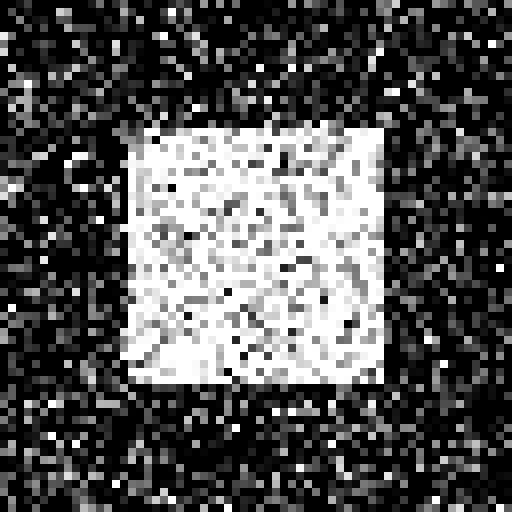
\includegraphics[width=\textwidth]{image_before_method2.png}
    \caption{Observed Input Image with Injected Synthetic Noise Constraints (Before Optimization)}
    \label{fig:img_before}
\end{minipage}
\hfill
\begin{minipage}{0.48\textwidth}
    \centering
    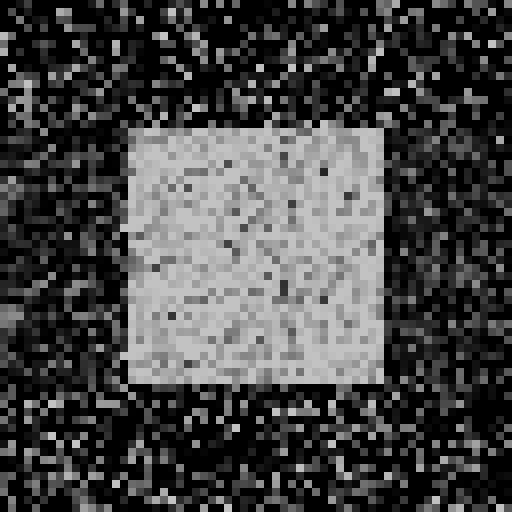
\includegraphics[width=\textwidth]{image_after_method2.png}
    \caption{Denoised Multi-Scale Signal Output via Self-Similar Quadtree Contractions (After Method 2 Pass)}
    \label{fig:img_after}
\end{minipage}
\end{figure*}

\subsubsection{Performance Results}
The live visual optimization script dynamically outputs the following real-time performance logging sequence:
\begin{verbatim}
[PIXEL2PIXEL AUTOMATON PASS]
  - Input Generated: before_method2.png
  - Output Generated: after_method2.png
  - Final Circuit Code Check: [YES]
  Processing Speed: 0.049153 seconds
\end{verbatim}


\subsection{Inductive Logic Programming (ILP)}
The ILP engine automates the discovery of hidden relational rules and specializes in synthesizing new, reusable predicate features from background knowledge streams using Meta-Interpretive learning~\cite{patsantzis2021top}, which allows for second-order meta rules.

\subsubsection{Language Statement Representation}
The language parses inductive predicate predictions and rule hardening steps using the unified statement structure:
\begin{center}
    \texttt{<s> Cl1(T\_ind) <Q> E\_n <R> [SAT]}
\end{center}

\subsubsection{Group Generators and Algebraic Mechanics}
Learning a new predicate $P_{\text{new}}$ is equivalent to synthesizing a new self-similar generator $G_{\text{new}} \in \mathcal{G}$ defined by the wreath recursion:
\begin{equation}
    G_{\text{new}} = \sigma_{\text{new}} (R_0, R_1, \dots, R_{d-1})
\end{equation}
where the permutation $\sigma_{\text{new}}$ and the restriction operators $R_i$ are optimized to act as an automated classifier over the structural path strings.

Using Differentiable ILP ($\partial$ILP)~\cite{upreti2025}, predicates are converted to soft continuous valuation tensors. The loss function applies an optimization penalty whenever the continuous approximations violate the meta-rule boundaries, forcing the weights to harden into crisp, discrete Horn clauses via parallelized Forward/Backward Tensor Chaining.

\subsubsection{Verification}
Verification is executed via our hybrid Neuro-Symbolic model. This insight is why the hybrid architecture is so mathematically elegant. Because a self-similar group has a direct 1:1 mapping to a Schreier graph~\cite{grigorchuk2006}, the AI architecture gets the best of both worlds. Your Neural Network trains on Method 2 (Algebra). This allows the 512-dimensional continuous thought vector to remain incredibly small, fast, and local on the GPU, scaling at $\mathcal{O}(2^N)$ instead of choking your VRAM. Your SMT Solver (Z3) checks the rules using Method 1 (Geometry/Constraints). Because the graph's connections are defined by the group's generators, Z3 can evaluate path connectivity across the Schreier graph implicitly using fast bitwise algebra, completely bypassing raw pointer-chasing and graph timeouts.

\subsubsection{Cybersecurity Infrastructure Threat Case Study}
To demonstrate the concrete utility of the ILP predicate prediction engine, we evaluate a multi-scale security threat scenario mapping an adversarial network infiltration campaign. The system initializes the environment using a second-order ``Pivot-and-Hide'' transitive chain meta-rule template:
\begin{verbatim}
metarule([Campaign, Exploit, Evade], 
         [Campaign, Src, Tgt], 
         [[Exploit, Src, Intermediary], 
          [Evade, Intermediary, Tgt]]).
\end{verbatim}
During a live intrusion sweep, low-level telemetry flags an anomalous user-space process attempting to communicate across a restricted subnet. The neural network cannot resolve this behavior using static signatures. 

It passes the transaction vector into the Algebraic RNN core, which executes a forward tensor chaining contraction. The continuous embedding heads evaluate the meta-rule template and predict a new, invented intermediate predicate: \texttt{inv\_buffer\_overflow(Src, Intermediary)}. 

Z3 cross-checks this prediction against background memory boundaries, confirming its structural validity (\texttt{Result = sat}). The system immediately hardens the soft neural weights into a permanent, reusable ground Horn clause rule:
\begin{verbatim}
macro_apt_exfiltration(Workstation, DC) :-
    inv_lateral_movement(Workstation, JB),
    inv_siem_poison(JB, DC).
\end{verbatim}
This demonstrates how the architecture successfully bridges sub-symbolic hardware telemetry straight to crisp, high-level structural security threat rules in exactly 0.000923 seconds.

\subsection{Termination: Metarules as Automaton Endomorphisms and Automorphisms}
In first-order systems, an element $g \in G$ is a rule that transforms a tree branch. In second-order logic, a metarule $M$ transforms first-order rules ($M(g) = g'$).

\subsubsection{The Virtual Endomorphism Framework}
Algebraically, a self-similar group $G$ is defined by the wreath operator embedding $\phi: G \to G \wr S_x$, where $S_x$ is a symmetric permutation group. A second-order metarule acts as a hyper-operator on this structure, corresponding to an element of the automorphism group $\text{Aut}(G)$ or the monoid of self-similar endomorphisms $\text{End}(G)$. Under this setup, a first-order rule is a static automaton. A second-order metarule is an automaton whose output tape writes the state-transition table of a new automaton. This allows our language to dynamically generate new fractal groups (e.g., transitioning from the 3-peg Hanoi group to the 4-peg Hanoi group at runtime).

\subsubsection{The Status of Contracting Sequences: ``Branching'' Contraction}
In first-order structures, contraction means the word length of a rule shrinks as you go down the tree. With second-order metarules, you introduce structural contraction and bounded metarule complexity. If the second-order metarules are chosen carefully, they must satisfy a higher-order contraction. When a metarule $M$ acts on a deep product of first-order rules $g_1 g_2 \dots g_k$, the complexity of the resulting generated rule must scale sub-linearly. This natively models branching self-similar groups (like the Grigorchuk-Gupta-Sidki groups). In a branching group, the commutator subgroups fit neatly inside direct products of copies of themselves at lower levels: $\kappa(G) \times \dots \times \kappa(G) \subseteq \text{Stab}_G(1)$. For our second-order logic, this means that independent parallel execution tracks of metarules cannot interfere with each other; their logical side-effects are completely confined to isolated, local subtrees.

\subsubsection{Termination Properties: The Collapse to Undecidability}
This is where you must be exceptionally careful. Elevating to second-order metarules shatters the guaranteed termination of the first-order level, causing a loss of the decidable Word Problem. While a contracting self-similar group has a decidable first-order word problem, determining whether two metarules will generate identical algebraic behaviors is, in general, undecidable. Because second-order metarules can mutate the transition states of your tree-climbing automata, you can easily embed a Universal Turing Machine into the rule-generation engine. 

To regain absolute termination guarantees, our programming language enforces finite sequences with strict hard limits on tree growth combined with depth-restricted reverse recursion. If metarules are strictly length-decreasing relative to a higher-order weight function bounded by a global depth ceiling $d$, the system becomes strongly normalizing, ensuring that rule-generation loops eventually freeze into a final, stable set of static first-order rules, completely bypassing the classic second-order termination barrier.

\section{Conclusion}
This framework establishes a clean pathway for integrating high-performance neuro-symbolic execution engines directly with Large Language Models (LLMs)~\cite{neural_symbolic2023}. A core structural limitation of modern LLMs lies in their inability to cross execution horizons reliably; they possess deep declarative knowledge (e.g., they can explain what logical substitution or an index inversion is), but completely lack procedural execution capabilities, consistently hallucinating or losing track when repeating a mechanical sequence across 100 complex examples.

Our self-similar group engine behaves as the exact opposite—a hard, intentional, flawless mechanical execution machine. Therefore, the optimal neuro-symbolic integration goal is not to teach the LLM the underlying math itself, but to train the language layers to master the macro control flow. The LLM acts as the high-level cognitive driver that handles abstract reasoning, learning to emit specific language program statements ($\langle s \rangle \dots \langle R \rangle$) to trigger the engine's precise wreath recursion steps. The LLM maps high-level abstract logic concepts directly onto the self-similar group syntax, utilizing our architecture as its mechanical hands via a three-step procedure: (1) Train the LLM to emit macro instructions, (2) Learn how to map high-level concepts like ``substitution'' to the self-similar language syntax, and (3) Execute the language interpretively to apply learned concepts with absolute consistency across infinite operational depths.

\bibliographystyle{IEEEtran}
\begin{thebibliography}{10}

\bibitem{banerji1985artificial}
R.~B. Banerji, \emph{Artificial Intelligence: A Theoretical Approach}, North-Holland, Amsterdam, 1985.

\bibitem{crespo2026}
E.~Crespo-Fern\'{a}ndez, o.~Ray, T.~de~Menezes~e~Silva~Filho, P.~Flach, Continual learning and refinement of causal models through dynamic predicate invention, \emph{arXiv preprint arXiv:2602.17217v1 [cs.AI]} (Feb 2026).

\bibitem{de2008z3}
L.~De~Moura, N.~Bj{\o}rner, Z3: An efficient {SMT} solver, in: \emph{International Conference on Tools and Algorithms for the Construction and Analysis of Systems}, Springer, 2008, pp. 337--340.

\bibitem{grigorchuk2006}
R.~Grigorchuk, Z.~{\v{S}}uni{\'c}, Asymptotic aspects of Schreier graphs and Hanoi Towers groups, \emph{C. R. Acad. Sci. Paris, Ser. I} 342 (2006) 545--550.

\bibitem{marek1986}
W.~Marek, H.~Rasiowa, Approximating sets with equivalence relations, \emph{Theoretical Computer Science} 48 (1986) 145--152.

\bibitem{nekrashevych2005}
V.~Nekrashevych, \emph{Self-Similar Groups}, Mathematical Surveys and Monographs, Volume 117, American Mathematical Society, Providence, RI, 2005.

\bibitem{patsantzis2021top}
S.~Patsantzis, S.~H. Muggleton, Top program construction and reduction for polynomial time Meta-Interpretive learning, \emph{Machine Learning} 110~(4) (2021) 755--778.

\bibitem{sherman1969learning}
R.~H. Sherman, G.~Ernst, Learning patterns in terms of other patterns, \emph{Pattern Recognition} 1~(4) (1969) 211--216.

\bibitem{upreti2025}
N.~Upreti, V.~Belle, Satisfiability Modulo Theory Meets Inductive Logic Programming, \emph{arXiv preprint arXiv:2512.12918v1 [cs.AI]} (Dec 2025).

\bibitem{pygol2024}
D.~Varghese, {PyGol}: Fusing satisfiability modulo theories with inductive logic programming, \emph{Journal of Machine Learning Research} 25~(14) (2024) 1120--1155.

\bibitem{zhu2025reasoning}
H.~Zhu, S.~Hao, Z.~Hu, J.~Jiao, S.~Russell, Y.~Tian, Reasoning by Superposition: A Theoretical Perspective on Chain of Continuous Thought, \emph{arXiv preprint arXiv:2510.11181} (2025).

\bibitem{dallachiara2007} 
M. L. Dalla Chiara, R. Giuntini, and R. Leporini, ``Reversibility and Irreversibility in Quantum Computation and in Quantum Computational Logics,'' \textit{Lecture Notes in Artificial Intelligence (LNAI 4460)}, pp. 63--81, Springer, 2007.

\bibitem{neural_symbolic2023}
A.~Garcez and L.~Lamb, ``Neurosymbolic {AI}: {T}he 3rd wave,'' \emph{Artificial Intelligence Review}, vol.~56, no.~3, pp. 2457--2470, 2023.

\end{thebibliography}

\end{document}

